% Options for packages loaded elsewhere
\PassOptionsToPackage{unicode}{hyperref}
\PassOptionsToPackage{hyphens}{url}
\PassOptionsToPackage{dvipsnames,svgnames,x11names}{xcolor}
%
\documentclass[
  singlecolumn,
  9pt]{article}

\usepackage{amsmath,amssymb}
\usepackage{iftex}
\ifPDFTeX
  \usepackage[T1]{fontenc}
  \usepackage[utf8]{inputenc}
  \usepackage{textcomp} % provide euro and other symbols
\else % if luatex or xetex
  \usepackage{unicode-math}
  \defaultfontfeatures{Scale=MatchLowercase}
  \defaultfontfeatures[\rmfamily]{Ligatures=TeX,Scale=1}
\fi
\usepackage[]{libertinus}
\ifPDFTeX\else  
    % xetex/luatex font selection
\fi
% Use upquote if available, for straight quotes in verbatim environments
\IfFileExists{upquote.sty}{\usepackage{upquote}}{}
\IfFileExists{microtype.sty}{% use microtype if available
  \usepackage[]{microtype}
  \UseMicrotypeSet[protrusion]{basicmath} % disable protrusion for tt fonts
}{}
\makeatletter
\@ifundefined{KOMAClassName}{% if non-KOMA class
  \IfFileExists{parskip.sty}{%
    \usepackage{parskip}
  }{% else
    \setlength{\parindent}{0pt}
    \setlength{\parskip}{6pt plus 2pt minus 1pt}}
}{% if KOMA class
  \KOMAoptions{parskip=half}}
\makeatother
\usepackage{xcolor}
\usepackage[top=30mm,bottom=30mm,left=20mm,heightrounded]{geometry}
\setlength{\emergencystretch}{3em} % prevent overfull lines
\setcounter{secnumdepth}{-\maxdimen} % remove section numbering
% Make \paragraph and \subparagraph free-standing
\ifx\paragraph\undefined\else
  \let\oldparagraph\paragraph
  \renewcommand{\paragraph}[1]{\oldparagraph{#1}\mbox{}}
\fi
\ifx\subparagraph\undefined\else
  \let\oldsubparagraph\subparagraph
  \renewcommand{\subparagraph}[1]{\oldsubparagraph{#1}\mbox{}}
\fi


\providecommand{\tightlist}{%
  \setlength{\itemsep}{0pt}\setlength{\parskip}{0pt}}\usepackage{longtable,booktabs,array}
\usepackage{calc} % for calculating minipage widths
% Correct order of tables after \paragraph or \subparagraph
\usepackage{etoolbox}
\makeatletter
\patchcmd\longtable{\par}{\if@noskipsec\mbox{}\fi\par}{}{}
\makeatother
% Allow footnotes in longtable head/foot
\IfFileExists{footnotehyper.sty}{\usepackage{footnotehyper}}{\usepackage{footnote}}
\makesavenoteenv{longtable}
\usepackage{graphicx}
\makeatletter
\def\maxwidth{\ifdim\Gin@nat@width>\linewidth\linewidth\else\Gin@nat@width\fi}
\def\maxheight{\ifdim\Gin@nat@height>\textheight\textheight\else\Gin@nat@height\fi}
\makeatother
% Scale images if necessary, so that they will not overflow the page
% margins by default, and it is still possible to overwrite the defaults
% using explicit options in \includegraphics[width, height, ...]{}
\setkeys{Gin}{width=\maxwidth,height=\maxheight,keepaspectratio}
% Set default figure placement to htbp
\makeatletter
\def\fps@figure{htbp}
\makeatother
% definitions for citeproc citations
\NewDocumentCommand\citeproctext{}{}
\NewDocumentCommand\citeproc{mm}{%
  \begingroup\def\citeproctext{#2}\cite{#1}\endgroup}
\makeatletter
 % allow citations to break across lines
 \let\@cite@ofmt\@firstofone
 % avoid brackets around text for \cite:
 \def\@biblabel#1{}
 \def\@cite#1#2{{#1\if@tempswa , #2\fi}}
\makeatother
\newlength{\cslhangindent}
\setlength{\cslhangindent}{1.5em}
\newlength{\csllabelwidth}
\setlength{\csllabelwidth}{3em}
\newenvironment{CSLReferences}[2] % #1 hanging-indent, #2 entry-spacing
 {\begin{list}{}{%
  \setlength{\itemindent}{0pt}
  \setlength{\leftmargin}{0pt}
  \setlength{\parsep}{0pt}
  % turn on hanging indent if param 1 is 1
  \ifodd #1
   \setlength{\leftmargin}{\cslhangindent}
   \setlength{\itemindent}{-1\cslhangindent}
  \fi
  % set entry spacing
  \setlength{\itemsep}{#2\baselineskip}}}
 {\end{list}}
\usepackage{calc}
\newcommand{\CSLBlock}[1]{\hfill\break#1\hfill\break}
\newcommand{\CSLLeftMargin}[1]{\parbox[t]{\csllabelwidth}{\strut#1\strut}}
\newcommand{\CSLRightInline}[1]{\parbox[t]{\linewidth - \csllabelwidth}{\strut#1\strut}}
\newcommand{\CSLIndent}[1]{\hspace{\cslhangindent}#1}

\usepackage{cancel}
\usepackage[noblocks]{authblk}
\renewcommand*{\Authsep}{, }
\renewcommand*{\Authand}{, }
\renewcommand*{\Authands}{, }
\renewcommand\Affilfont{\small}
\usepackage{cancel}
\makeatletter
\@ifpackageloaded{caption}{}{\usepackage{caption}}
\AtBeginDocument{%
\ifdefined\contentsname
  \renewcommand*\contentsname{Table of contents}
\else
  \newcommand\contentsname{Table of contents}
\fi
\ifdefined\listfigurename
  \renewcommand*\listfigurename{List of Figures}
\else
  \newcommand\listfigurename{List of Figures}
\fi
\ifdefined\listtablename
  \renewcommand*\listtablename{List of Tables}
\else
  \newcommand\listtablename{List of Tables}
\fi
\ifdefined\figurename
  \renewcommand*\figurename{Figure}
\else
  \newcommand\figurename{Figure}
\fi
\ifdefined\tablename
  \renewcommand*\tablename{Table}
\else
  \newcommand\tablename{Table}
\fi
}
\@ifpackageloaded{float}{}{\usepackage{float}}
\floatstyle{ruled}
\@ifundefined{c@chapter}{\newfloat{codelisting}{h}{lop}}{\newfloat{codelisting}{h}{lop}[chapter]}
\floatname{codelisting}{Listing}
\newcommand*\listoflistings{\listof{codelisting}{List of Listings}}
\makeatother
\makeatletter
\makeatother
\makeatletter
\@ifpackageloaded{caption}{}{\usepackage{caption}}
\@ifpackageloaded{subcaption}{}{\usepackage{subcaption}}
\makeatother
\ifLuaTeX
  \usepackage{selnolig}  % disable illegal ligatures
\fi
\IfFileExists{bookmark.sty}{\usepackage{bookmark}}{\usepackage{hyperref}}
\IfFileExists{xurl.sty}{\usepackage{xurl}}{} % add URL line breaks if available
\urlstyle{same} % disable monospaced font for URLs
\hypersetup{
  pdftitle={Measurement Bias in Causal Inference: Advice for Evolutionary Human Scientists},
  pdfauthor={Joseph A. Bulbulia},
  pdfkeywords={DAGS (Directed Acyclic Graphs), Causal
Inference, Confounding, History, Psychology, Panel},
  colorlinks=true,
  linkcolor={blue},
  filecolor={Maroon},
  citecolor={Blue},
  urlcolor={Blue},
  pdfcreator={LaTeX via pandoc}}

\title{Measurement Bias in Causal Inference: Advice for Evolutionary
Human Scientists}


  \author{Joseph A. Bulbulia}
            \affil{%
                  Victoria University of Wellington, New Zealand, School
                  of Psychology, Centre for Applied Cross-Cultural
                  Research
              }
      
\date{2023-11-16}
\begin{document}
\maketitle
\begin{abstract}
This article explains the concept of measurement bias.
\end{abstract}
In this article, we use causal diagrams to illustrate the distinct
pathway of bias introduced by measurement error and discuss its
implications for research design. Unlike confounding bias (CITE), which
arises from the presence of a common cause of both the exposure and the
outcome, and selection bias, which arises from the participant selection
process or dropout rate (CITE), measurement bias arises from how
variables are measured or categorised.

\subsubsection{Measurement Error in the
Confounder}\label{measurement-error-in-the-confounder}

Measurement error pervades all human research. Figure
Figure~\ref{fig-dag-measure-confounder} demonstrates that even
error-free measurements of the exposure and outcome cannot counteract
the bias in causal effect estimates introduced by measurement error in
the confounders. Accurate measurement of confounders mitigates threats
to confounding. Once more, conducting a sensitivity analysis is
essential to evaluate the potential impact of this threat.\footnote{A
  simple yet powerful form of sensitivity analysis involves the
  computation of E-Values. E-Values calculate the minimal strength of
  association that an unmeasured confounder would require with both the
  exposure and outcome, beyond the measured confounders, to negate the
  observed exposure-outcome association (refer to the R package
  \texttt{EValue}:(\citeproc{ref-mathur2018}{Mathur \emph{et al.}
  2018})).}

\begin{figure}

\centering{

\includegraphics[width=0.6\textwidth,height=\textheight]{notes-on-measurement-bias_files/figure-pdf/fig-dag-measure-confounder-1.pdf}

}

\caption{\label{fig-dag-measure-confounder}Causal diagram showing a
confounder, L, measured with error, L'. Despite perfect measurements of
the exposure, A, and the outcome, Y, a bias-inducing (backdoor) path
opens between A - L - Y, highlighted in red. Given the ubiquity of
measurement error, it is imperative to minimise such errors and conduct
sensitivity analyses to assess the risk of unmeasured confounding.}

\end{figure}%

Acknowledging the pervasiveness of measurement error and its potential
influence on our research, we will further explore how structural
approaches to understanding measurement error clarify the nature of the
problem, methods for adjustment, and the unceasing need for sensitivity
analyses.

Following Hernán and Cole (\citeproc{ref-hernuxe1n2009}{2009}), we
define structural concepts of measurement error and utilise causal
diagrams to understand how such errors may bias causal effect estimates.
A deeper understanding of these concepts (developed in
(\citeproc{ref-vanderweele2012}{VanderWeele and Hernán 2012}), will
equip us to better manage and account for assessing bias from
measurement error in causal inference.

\subsubsection{1. Uncorrelated non-differential (undirected) measurement
error}\label{uncorrelated-non-differential-undirected-measurement-error}

As shown in Figure~\ref{fig-dag-uu-null}, an uncorrelated
non-differential measurement error occurs when the errors in the
measurement of the exposure and outcome are not related.

To clarify, consider again the task of estimating the causal effect of
beliefs in Big Gods on social complexity. Suppose ancient societies
randomly omitted or recorded details about both beliefs in Big Gods and
indicators of social complexity in their records. Alternatively, suppose
that such records were not preserved equally across cultures for reasons
unrelated to these parameters. In this case, errors in the documentation
of both variables would be random. The errors would not be related to
the intensity of the beliefs in Big Gods or the level of social
complexity. The structure of this example of uncorrelated and
non-differential error is presented in Figure~\ref{fig-dag-uu-null}.

Uncorrelated non-differential measurement error does not create bias
under the null. As evident from Figure~\ref{fig-dag-uu-null},
d-separation is preserved. Equivalently, there are no open backdoor
paths on the graph. However, when there is an actual effect of the
exposure on the outcome, non-differential measurement error generally
leads to attenuated effect estimates. For this reason, uncorrelated
non-differential measurement error can be problematic for causal
inference even though they do not induce structural bias under the null.

\begin{figure}

\centering{

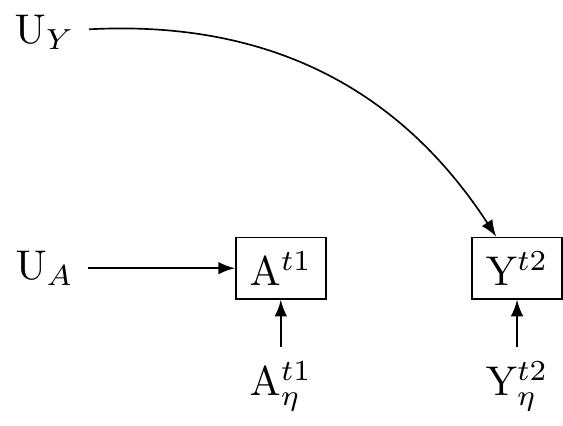
\includegraphics[width=0.6\textwidth,height=\textheight]{notes-on-measurement-bias_files/figure-pdf/fig-dag-uu-null-1.pdf}

}

\caption{\label{fig-dag-uu-null}Uncorrelated non-differential
measurement error does not bias estimates under the null, however may
attenuate true effects.}

\end{figure}%

\subsubsection{2. Uncorrelated differential (directed) measurement
error}\label{uncorrelated-differential-directed-measurement-error}

As shown in Figure~\ref{fig-dag-indep-d-effect}, uncorrelated
differential (or directed) measurement error occurs when the measurement
errors are related to the level of exposure or outcome but not to each
other. For instance, societies with stronger beliefs in Big Gods might
have more or less detailed records of social complexity. Suppose that,
in the absence of any intervention on beliefs in Gods, there is no
association between the measurement errors. Here, the errors are
differential as they depend on the intensity of religious beliefs but
are uncorrelated as the errors in documenting beliefs in Big Gods and
social complexity are otherwise independent. Uncorrelated differential
(or directed) measurement error is presented in
Figure~\ref{fig-dag-indep-d-effect} and leads to bias under the null,
indicated by the red path. Equivalently, we may say that uncorrelated
differential (or directed) measurement error opens a backdoor path
between the exposure and the outcome.

Note that the bias presented in Figure~\ref{fig-dag-indep-d-effect}, an
example of directed measurement error, also describes the bias we
considered when there is panel attrition and which the exposure affects
selection (CITE). In that scenario, the outcome in the selected group is
measured with error -- it no longer represents the measurement of the
outcome in the source population at baseline -- furthermore, this error
is affected by exposure. The previous example described bias in
estimation from the vantage point of collider stratification; however,
we can also explain the distortion as directed measurement bias.

\begin{figure}

\centering{

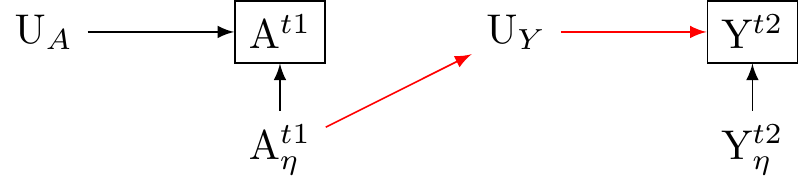
\includegraphics[width=1\textwidth,height=\textheight]{notes-on-measurement-bias_files/figure-pdf/fig-dag-indep-d-effect-1.pdf}

}

\caption{\label{fig-dag-indep-d-effect}Directed independent
(uncorrelated) measurement error can bias effect estimates under the
null. This bias is indicated by the red paths.}

\end{figure}%

\subsubsection{3. Correlated non-differential (undirected) measurement
error}\label{correlated-non-differential-undirected-measurement-error}

As shown, Figure~\ref{fig-dag-dep-u-effect} correlated non-differential
(undirected) measurement error occurs when the errors in measuring both
the exposure and outcome are related independently of the exposure. The
scenario is presented in Figure~\ref{fig-dag-dep-u-effect}. Imagine that
some societies had more advanced record-keeping systems that resulted in
more accurate and detailed accounts of both beliefs in Big Gods and
social complexity. Furthermore, imagine that record keepers provide
better information about religious beliefs. In this case, the errors
between beliefs in Big Gods and social complexity are correlated because
the accuracy of records for both variables is influenced by the same
underlying factor (the record-keeping abilities). However, the errors
are not directed insofar as levels of religious beliefs and social
complexity do not affect the assumed bias in record keeping. Correlated
non-differential measurement error may induce bias under the null,
indicated by the red path in Figure~\ref{fig-dag-dep-u-effect}.

\begin{figure}

\centering{

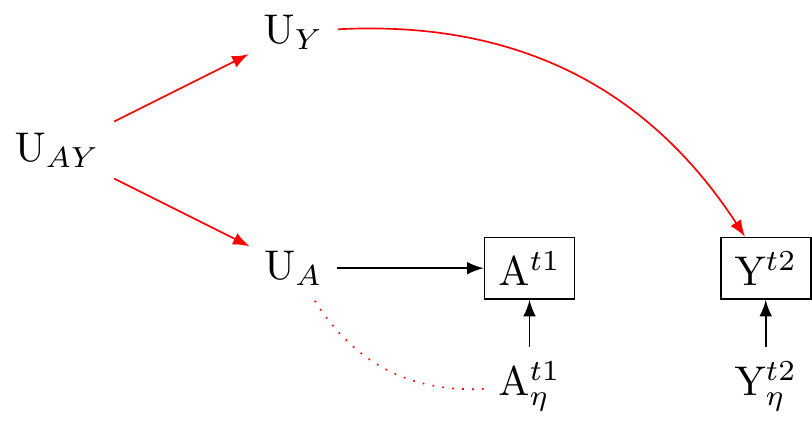
\includegraphics[width=0.8\textwidth,height=\textheight]{notes-on-measurement-bias_files/figure-pdf/fig-dag-dep-u-effect-1.pdf}

}

\caption{\label{fig-dag-dep-u-effect}Correlated undirected measurement
error can distort causal effect estimates under the null, indicated by
the red path.}

\end{figure}%

\subsubsection{4. Correlated differential (directed) measurement
error}\label{correlated-differential-directed-measurement-error}

Correlated differential (directed) measurement error occurs when the
measurement errors are related independently of the exposure, and the
exposure also affects levels of these correlated error terms. The
structure of this bias is presented in Figure~\ref{fig-dag-d-d}. Suppose
societies with stronger beliefs in Big Gods tend to record their
religious beliefs and social structures more meticulously than others.
Suppose further that religious elites conduct this record-keeping. The
errors may be both correlated and differential if societies with beliefs
in Big Gods tend to favour these religious elites, leading to biased
records.

Consider further the three-wave panel design, where we aim to estimate
the effect of self-reported religious service attendance on
self-reported monthly donations to charity. A set of confounders is
included at baseline, comprising previous measures of religious service
attendance and monthly donations to charity. Because our measures rely
on self-reports, they may be especially prone to measurement error.

Assume there is an unmeasured common cause affecting both the
measurement error of religious service attendance and the measurement
error of donations to charity. This bias might occur if individuals
consistently over- or under-report their religious service attendance
and donations due to social desirability bias.

In Part 3, we discussed how including the exposure measured at baseline
can reduce confounding in a three-wave panel design. By controlling for
the baseline exposure, we effectively adjust for any static
characteristics that cause a correlation between the exposure and
outcome. Taking this further, including baseline measures in the
analysis might mitigate the impact of measurement errors on causal
effect estimation, provided the errors meet specific conditions.

Consider a study with two time points: baseline and follow-up. Let
\(A_0\) and \(A_1\) represent the true exposure levels at baseline and
follow-up, respectively, and \(Y_0\) and \(Y_2\) represent the true
outcomes at these respective time points. In practice, the observed or
measured values may differ from the true values due to measurement
error. We use primes to denote these measured values:

\begin{itemize}
\tightlist
\item
  \(A'_0 = A_0 + UA_0\)
\item
  \(A'_1 = A_1 + UA_1\)
\item
  \(Y'_0 = Y_0 + UY_0\)
\item
  \(Y'_2 = Y_2 + UY_2\)
\end{itemize}

Here, \(UA_0\), \(UA_1\), \(UY_0\), and \(UY_2\) are the additive
measurement errors for exposure and outcome at baseline and follow-up,
respectively. The primes on \(A\) and \(Y\) symbolise the values as they
are observed, reflecting their true values and the corresponding
measurement errors.

By including \(A'_0\) and \(Y'_0\) as covariates, we aim better identify
the incidence effect of a change in exposure from baseline to follow-up
on the outcome. However, to mitigate bias arising from correlated
measurement errors, the following conditions must hold:

\begin{itemize}
\tightlist
\item
  The expectation of the measurement errors is consistent over time:
  \(E(UA_0) = E(UA_1)\) and \(E(UY_0) = E(UY_2)\).
\item
  The conditional correlation between the errors is zero given baseline
  measures: \(Cov(UA_1, UY_2) = 0 | A'_0,Y'_0,L'_0\).
\end{itemize}

Including measurements of the baseline exposure and baseline outcome can
reduce undirected measurement errors, but the strategy require that the
errors are both constant over time and undirected. If the errors vary
over time or if the the exposure affects the error of the outcome then
controlling for baseline measurements of the exposure and outcome will
be inadequate for confounding control (see:
(\citeproc{ref-keogh2020}{Keogh \emph{et al.} 2020})).

Consider a scenario where individuals attending religious services at
wave 1 acquire greater social desirability bias, affecting their
reporting. If the outcome at wave 2 is charitable giving, this bias
could distort the real level of giving. Directed measurement bias could
falsely link the increase in charity to religious service attendance,
masking the true effect of over-reporting due to social desirability
bias.

In short, controlling for baseline exposure, while powerful for
confounding control, is not a panacea. Confounding control requires
careful consideration of the quality of measures across time and may
require further steps, such as changing the wording of questions, to
mitigate directed measurement error bias. For example, to bypass
presentation bias, questions about charity from presentation bias that
is affected by the exposure may focus on \emph{received help} rather
than \emph{offered help}. This approach assumes that a more altruistic
religious community would lead to a higher probability of receiving
help, that the measure is relatively accurate, and that biases in
reporting do not differ by exposure status.

\begin{figure}

\centering{

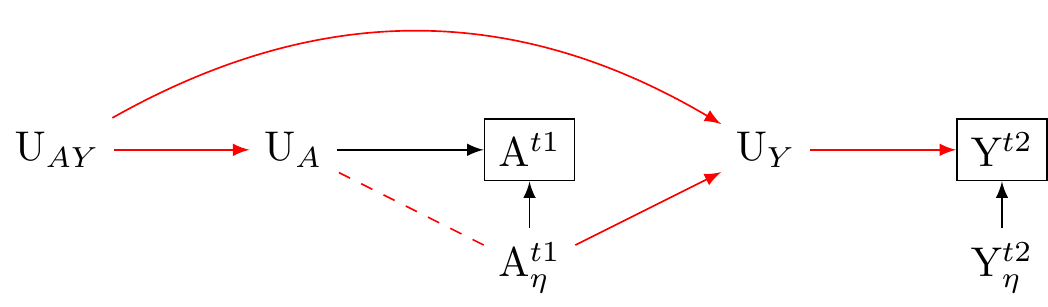
\includegraphics[width=1\textwidth,height=\textheight]{notes-on-measurement-bias_files/figure-pdf/fig-dag-d-d-1.pdf}

}

\caption{\label{fig-dag-d-d}Directed dependent (correlated) measurement
error leads to bias in causal effect estimates. Here, the exposure
affects the measurement error of the outcome. Additionally, the
measurement error of the exposure and outcome are correlated. These
dynamics open pathways for bias, indicated by the red paths. Sructural
sources of bias in measurement error must be evaluated, and sensitivity
analyses should be preformed to assess threats to causal inference.}

\end{figure}%

\subsubsection{Using time-ordered causal diagrams to understand threats
of correlated measurement error for causal inference comparative
cultural
research}\label{using-time-ordered-causal-diagrams-to-understand-threats-of-correlated-measurement-error-for-causal-inference-comparative-cultural-research}

To comprehend the structural features that might undermine causal
inferences in comparative cultural research, consider a simplified
scenario. Imagine that before conducting cultural comparisons, the
measurement errors of the exposure and outcome variables are
uncorrelated, as illustrated in Figure~\ref{fig-dag-uu-null}. While
measurement error can lead to a downward bias off the null, under the
null, no bias occurs.

However, when selecting study participants from different cultures --
cultures that inherently vary in interpretations and behaviours --- an
unmeasured bias under the null can occur, as shown in
Figure~\ref{fig-dag-dep-u-effect-selection}. To highlight this issue, we
modify the causal diagram in Figure~\ref{fig-dag-uu-null} to include
participant selection. This act of comparative selection creates a new
study population in which the error terms of measures become associated.
We cannot condition on cultural membership to block these associations,
as it was the act of conditioning that induced them in the new study
population.

If we did not undertake comparative sampling, the exposure and outcome
would be d-separated under the given scenario, yielding no bias for
separate studies, as shown in Figure~\ref{fig-dag-uu-null}. We cannot
resort to stratifying on culture to address this bias, as it is the act
of stratifying on culture that gives rise to correlated measurement
errors. Conducting separate analyses by culture precludes
generalisation, yet science seeks to find generalisations wherever it
can. Human scientists strive to identify functions supporting
transportable inferences wherever possible (see Part 2).

Yet, given the myriad ways the true structures of the world can align
with correlational models, we must be cautious when using conventional
invariance testing thresholds as the arbiters for cultural science. Such
tests should be considered exploratory tools. They can guide comparative
research, but must not replace careful scientific thinking, informed by
local expertise. In causal inference, decisions must be tailor-made to
fit the specific situation at hand.

\begin{figure}

\centering{

\includegraphics[width=1\textwidth,height=\textheight]{notes-on-measurement-bias_files/figure-pdf/fig-dag-dep-u-effect-selection-1.pdf}

}

\caption{\label{fig-dag-dep-u-effect-selection}This figrue illustrates
the introduction of measurement bias in comparative cross-cultural
research. Selection at the baseline stage induces correlations in the
exposure and outcome measurement errors, shown by red paths. The figure
underscores the importance of clearly defining the source populationand
the target population; in many comparative studies, the source
population cannot coherently map onto any coherent targe population.
Reserachers will often do better to restrict generalisations within
cultures.}

\end{figure}%

\subsubsection{Using time-ordered causal diagrams to understand how
post-outcome adjustment may diminish threats of directed measurement
error in cultural evolutionary
research}\label{using-time-ordered-causal-diagrams-to-understand-how-post-outcome-adjustment-may-diminish-threats-of-directed-measurement-error-in-cultural-evolutionary-research}

Figure Figure~\ref{fig-dag-measure-selection-0} illustrates a situation
often encountered in the evolutionary science of historical cultures.
Let us assume that there is no relationship between the actual exposure,
\(A\), and actual outcome, \(Y\). Further, suppose that the outcome
influences the measurement error of the exposure, denoted as \(UA\).
This influence is assumed to be directional, opening a backdoor path
between the measured exposure, \(A^{\prime}\), and the measured outcome,
\(Y'\). (For simplicity, we will not consider that the outcome is
measured with error; this assumption does not alter the problem's
structure.) Scenarios akin to that shown in
Figure~\ref{fig-dag-measure-selection-0} frequently emerge in historical
evolutionary human science because history written by victors.

\begin{figure}

\centering{

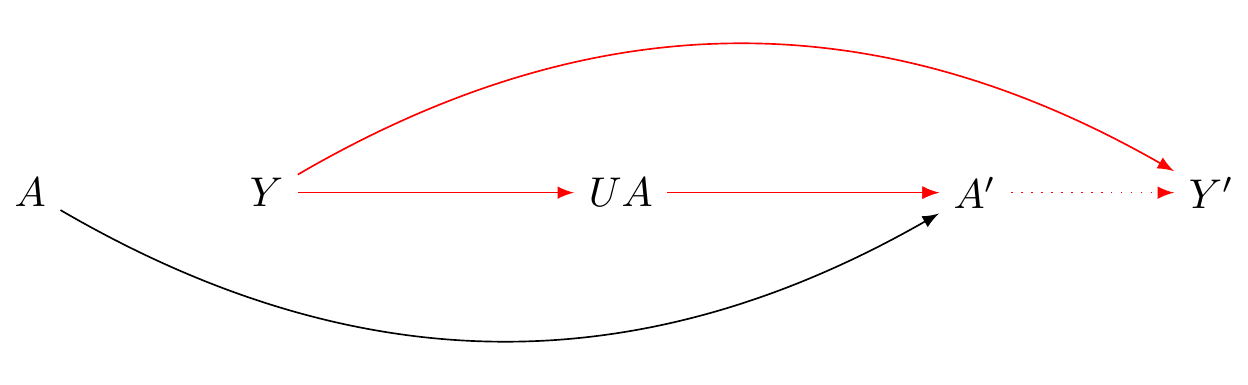
\includegraphics[width=1\textwidth,height=\textheight]{notes-on-measurement-bias_files/figure-pdf/fig-dag-measure-selection-0-1.pdf}

}

\caption{\label{fig-dag-measure-selection-0}The figure illustrates the
bias arising measurement error of A' caused by Y. Although A and Y are
independent, their measured counterparts, A' and Y', are not. The
systematic error introduced by changes in Y opens a biasing path,
signified in red.}

\end{figure}%

Figure~\ref{fig-dag-measure-selection} exposes the structure of bias
where post-outcome adjustment is necessary to mitigate or eliminate
measurement bias instigated by the outcome itself. Assume our interest
lies in quantifying the influence of belief in Big gods on social
complexity. We assumed that highly complex societies amend history,
eliminating traces of beliefs in lesser gods. If traces of beliefs in
lesser gods were recoverable through sources such as language, cultural
evolutoinary researchers would obtain better effect estimates.
Figure~\ref{fig-dag-measure-selection} clarifies the intuition that
recovering echoes of the silenced is worthwhile for enhancing the
accuracy of our causal effect estimates.

\begin{figure}

\centering{

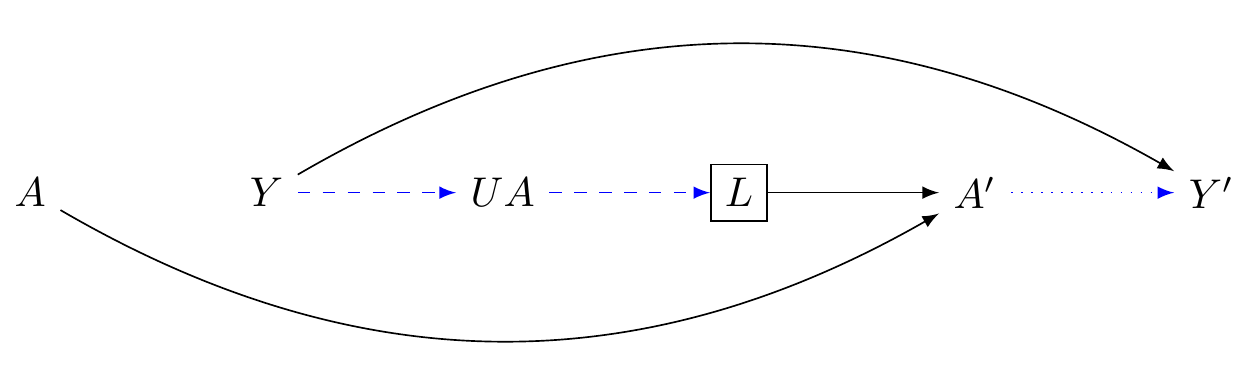
\includegraphics[width=1\textwidth,height=\textheight]{notes-on-measurement-bias_files/figure-pdf/fig-dag-measure-selection-1.pdf}

}

\caption{\label{fig-dag-measure-selection}Causal diagram elucidates how
refined measurements attenuate bias. By recovering measures undistorted
by past outcomes, we attenuate the directed measurement error. We
repesent this scenario on the graph by removing the path from Y to UA.}

\end{figure}%

\subsubsection{Using time-ordered causal diagrams to clarify the
structural assumptions of latent factor
models}\label{using-time-ordered-causal-diagrams-to-clarify-the-structural-assumptions-of-latent-factor-models}

Human evolutionary scientists who wish to collect time-series data by
measuring individuals over time in panel designs may consider using
multi-item constructs in their panel studies. What are the implications
of doing so? Multi-item constructs have long been favoured by
traditional psychometric theory. However, classical psychometric theory
developed without the benefit of causal approaches. VanderWeele argues
that difficulties surface when assessing the causal assumptions of
formative and reflective latent factor models
(\citeproc{ref-vanderweele2022}{VanderWeele 2022}). These models are
based on statistical formulations. However, the causal inferences they
embody cannot be determined solely by statistical models. This
discussion will concentrate on reflective models, although the concerns
raised are equally applicable to formative models, and I refer
interested readers to: (\citeproc{ref-vanderweele2022}{VanderWeele
2022}).\footnote{In formative models, observed variables are perceived
  to generate the latent variable. This latent variable is assumed to be
  a composite of the observed variables, \(X_i\), mathematically
  expressed as \(\eta = \sum_i\lambda_i X_i\). The structural assumption
  is that a single latent variable causally influences the observed
  variables. This structural is depicted in
  Figure~\ref{fig-structural-assumptions-reflective-model}.}

\begin{figure}

\centering{

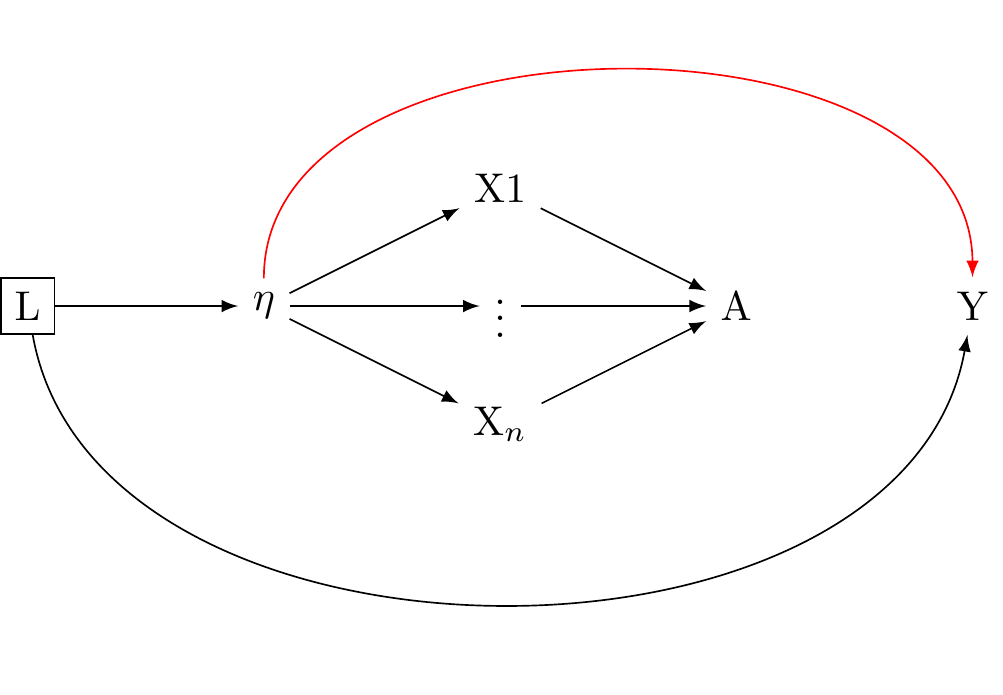
\includegraphics[width=0.8\textwidth,height=\textheight]{notes-on-measurement-bias_files/figure-pdf/fig-structural-assumptions-reflective-model-1.pdf}

}

\caption{\label{fig-structural-assumptions-reflective-model}Structural
assumptions of the reflective model imply a univariate reality causes
the outcome. These assumptions are strong because they exclude
multivariate causes of the indicators for constructs, as well as
independent effects of the indicators on outcomes. Blue line indicates
assumed causal path. The figure is adapted from VanderWeele 2022.}

\end{figure}%

However, VanderWeele notes that the statistical model is consistent with
multiple causal models. The presumption that a univariate latent reality
underlies the reflective (and formative) latent factor models is a
stronger assumption than previously acknowledged. For example, an
alternative structural model equally compatible with the data is
presented in Figure~\ref{fig-dag-multivariate-reality-again} Here,
multivariate reality gives rise to the indicators from which we draw our
measures. Indeed, for specific widely used measures, the assumption of a
univariate reality is so strong that they make testable assumptions.
VanderWeele and Vansteeland test the empirical examination assumptions
of widely used depression scales and find the assumptions fail
(\citeproc{ref-vanderweele2022b}{VanderWeele and Vansteelandt 2022}).
Although we cannot generally determine which structural models are
accurate, the data rule out the univariate model in the case that
VanderWeele and Vansteelandt (\citeproc{ref-vanderweele2022b}{2022})
examine.

\begin{figure}

\centering{

\includegraphics[width=0.6\textwidth,height=\textheight]{notes-on-measurement-bias_files/figure-pdf/fig-dag-multivariate-reality-again-1.pdf}

}

\caption{\label{fig-dag-multivariate-reality-again}Vanderweele's example
of an alternative structural model that is consistent with the
statistical model that underpins reflective construct models. Here, a
multivariate reality gives rise to the indicators from which we draw our
measures. Additional paths from the latent factors to the outcome are
presented in Blue. (Confounders are omited for simplicity). This figure
is adapted from VanderWeele 2022.}

\end{figure}%

Although the assumptions of a univariate reality that underlie
traditional latent factor models are not generally credible, VanderWeele
suggests that construct measures can still find application in research.
On VanderWeele's view, the key to salvaging latent factor models is to
extend the theory of causal inference under multiple interventions to
latent factor models (\citeproc{ref-vanderweele2022}{VanderWeele 2022}).
Specifically, by framing measured variables as functions of indicators
that may map onto a complex multivariate underlying reality, we may
approach them as coarsened indicators for that reality. As long as the
potential outcomes of these coarsened indicators are conditionally
independent of their treatment assignments and there is no unmeasured
confounding, we may assume the constructs to consistently estimate the
causal effects of the complex reality that gives rise to them.

Although we may agree with VanderWeele that the theory of causal
inference under multiple interventions might offer some redemption to
factor models, we might still exercise caution when using construct
measures. Similar to the theory of causal inference under multiple
versions of treatments, there are situations where guaranteeing
conditional exchangeability might be unfeasible. Furthermore, even when
such assurance is possible, difficulties might arise in interpreting the
results or endorsing policy interventions. In the following section, I
develop a related concern arising from threats to confounding arising
from directed measurement error from the potentially multivariate
reality that underlies construct measures.

\subsubsection{Causal diagrams highlight biases arising from measurement
errors within
constructs}\label{causal-diagrams-highlight-biases-arising-from-measurement-errors-within-constructs}

Consider a three-wave panel with the assumption that no unmeasured
confounding exists. We represent the exposure \(A\) as a function of
indicators, \(A_{f(A_1, A_2, ..., A_n)}\), representing a coarsened
state of a multivariate reality. Each component of this reality
corresponds to a structural element, represented as
\(\eta_{A_1}, \eta_{A_2}, ..., \eta_{A_n}\), each with associated error
terms, \(U\eta_{A_1}, U\eta_{A_2}, ..., U\eta_{A_n}\).

We can similarly conceptualise the outcome \(Y\), as a function of
indicators, \(Y_{f(Y_1, Y_2, ..., Y_n)}\), representing a latent
reality. This latent reality is composed of the components
\(\eta_{Y_1}, \eta_{Y_2}, ..., \eta_{Y_n}\), each with their
corresponding error terms
\(U\eta_{Y_1}, U\eta_{Y_2}, ..., U\eta_{Y_n}\). For simplicity, we leave
out baseline confounders and imagine a randomised experiment.

Figure~\ref{fig-dag-coarsen-measurement-error} depicts this assumed
reality and outlines potential confounding paths due to directed
measurement error from the indicators of the exposure, measured with
error, to the indicators or the outcome, measured with error. Each path
consists of a structural component \(\eta_{A_n}\) and its associated
error term \(U\eta_{Y_n}\). We identify three potential confounding
paths resulting from directed measurement error.

The potential for confounding from measurement error in panel designs
fundamentally relies on the relationships and dependencies among
variables, not their quantity. However, it is worth emphasising that, in
theory, an increase in the number of latent states or error terms may
enhance the potential for confounding. Under simplifying assumptions,
the potential direct paths from the exposure to the outcome are given by
the product of the number of components of the exposure and the number
of error terms associated with the outcome, symbolically represented as
\(\eta A_n \times U\eta_{Y_n}\). In this simplified scenario, each
latent variable connected to exposure could influence every error term
of an outcome, creating a complex network of confounding paths.

Causal diagrams, when applied to measurement error in latent factor
models, underscore the necessity of thorough scrutiny of construct
measures in evolutionary human sciences. Although no universal rule
exists, researchers may sometimes choose to use single-item measures.
Each case, however, requires a meticulous investigation of the items'
definitions, probable interpretations, and potential causal implications
over time. Composite scales can enhance efficiency. If their underlying
assumptions make sense, it is sensible to use them. Yet, often these
assumptions will not hold. Human evolutionary scientists -- as well as
other human scientists -- need to cultivate the habits for evaluating
the specifics of each research question within its context.

\begin{figure}

\centering{

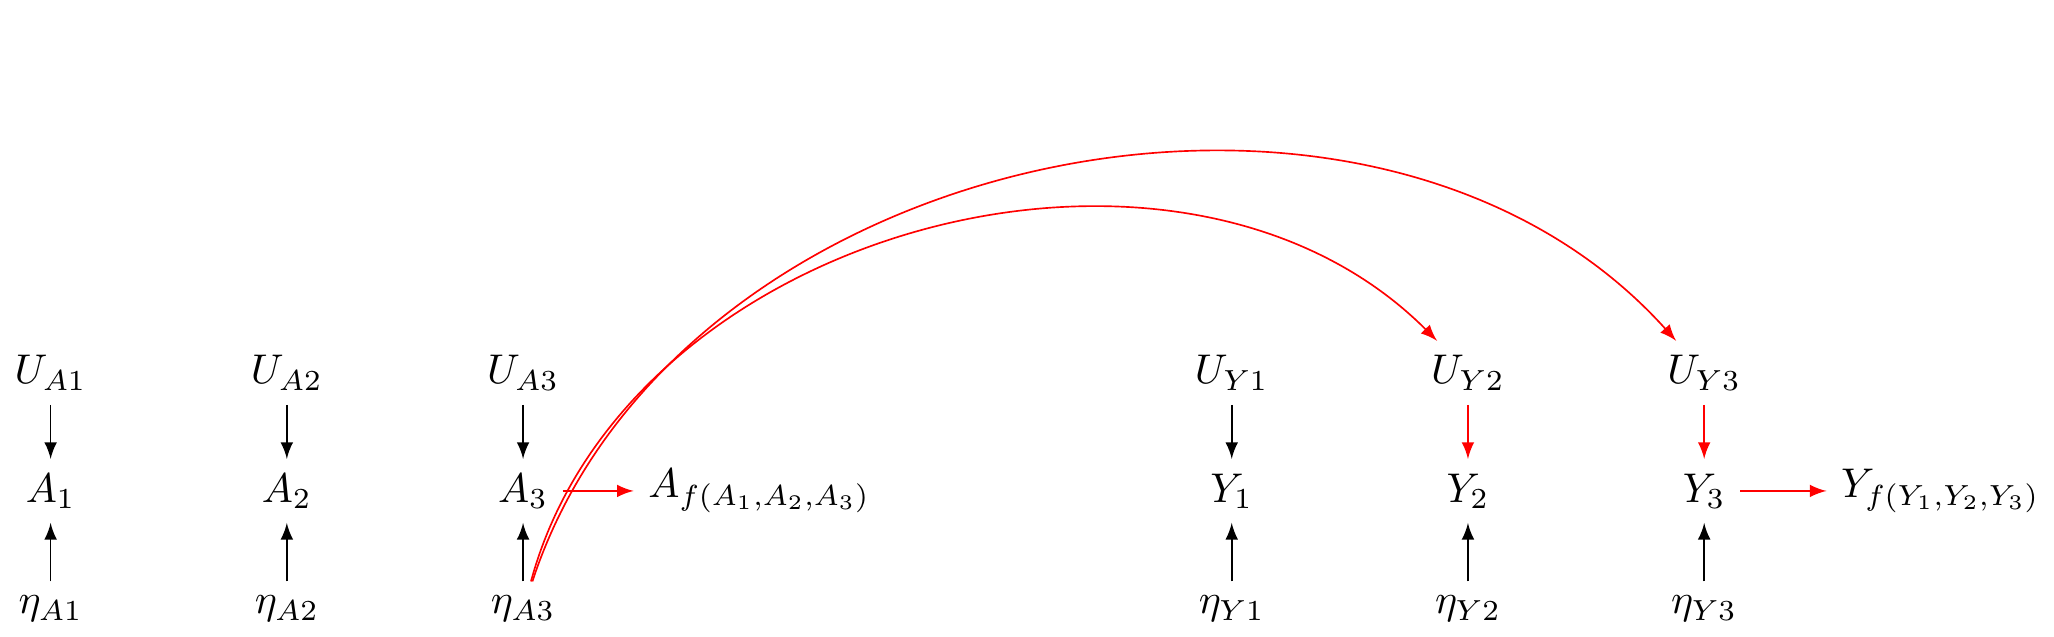
\includegraphics[width=1\textwidth,height=\textheight]{notes-on-measurement-bias_files/figure-pdf/fig-dag-coarsen-measurement-error-1.pdf}

}

\caption{\label{fig-dag-coarsen-measurement-error}Correlated, undirected
measurement error distorts causal effect estimates under the null,
depicted by the red path. This distortion is a potential issue with
multi-item factor models. Their popularity notwithstanding, a careful
consideration of measurement bias underscores the necessity to tailor
measurement strategies to specific research contexts.}

\end{figure}%

\subsubsection{Summary}\label{summary}

We describe sources of bias from measurement error in repeated measures
data designs. We examined four types of measurement error bias,
assessing how each might skew inference. Although adjustments for the
baseline exposure and baseline outcome can reduce confounding -- and
isolate incidence effects -- the strategy is not a panacea. Often the
exposure, or the source of error in its measurement, may plausibly
affect the measurement of the outcome. In such cases, the correlations
we obtain may be biased indicators of causation.

A host of useful resources exists for addressing measurement error,
including the works of Keogh \emph{et al.}
(\citeproc{ref-keogh2020}{2020}) Buonaccorsi
(\citeproc{ref-buonaccorsi2010}{2010}) Shi \emph{et al.}
(\citeproc{ref-shi2021}{2021}) Valeri \emph{et al.}
(\citeproc{ref-valeri2014}{2014}) and Bandalos
(\citeproc{ref-bandalos2018}{2018}). Additionally, specialist knowledge
may often indicate the direction of influence in the associations of
measurement error terms, whether positive or negative
(\citeproc{ref-suzuki2020}{Suzuki \emph{et al.} 2020};
\citeproc{ref-vanderweele2007a}{VanderWeele and Robins 2007},
\citeproc{ref-vanderweele2010}{2010}). In such cases, researchers may
sometimes employ causal diagrams with signed paths to improve causal
inferences (\citeproc{ref-vanderweele2012}{VanderWeele and Hernán
2012}). Such methods take us beyond the purpose of this section, which
has been to review how causal diagrams can be used to reveal sources of
counfounding from measurement bias, how measurement bias arises in
settings of comparative cultural research, why the latent factor models
employed to validate construct measures make exceptionally strong causal
claims, and why in some cases single item measures might do better.
Chronologically ordered causal diagrams, once more, disclose imperatives
not only for data analysis but also for data collection. They underscore
the need to devise and use measurement tools that minimise error. And
they empower us to reject blind adherence to psychometric tradition by
contemplating causality in the context of a specific question at hand.

\subsubsection*{References}\label{references}
\addcontentsline{toc}{subsubsection}{References}

\phantomsection\label{refs}
\begin{CSLReferences}{1}{0}
\bibitem[\citeproctext]{ref-bandalos2018}
Bandalos, DL (2018) \emph{Measurement theory and applications for the
social sciences}, Guilford Publications.

\bibitem[\citeproctext]{ref-buonaccorsi2010}
Buonaccorsi, JP (2010) \emph{Measurement error: Models, methods, and
applications}, New York: Chapman; Hall/CRC.
doi:\href{https://doi.org/10.1201/9781420066586}{10.1201/9781420066586}.

\bibitem[\citeproctext]{ref-hernuxe1n2009}
Hernán, MA, and Cole, SR (2009) Invited commentary: Causal diagrams and
measurement bias. \emph{American Journal of Epidemiology},
\textbf{170}(8), 959--962.
doi:\href{https://doi.org/10.1093/aje/kwp293}{10.1093/aje/kwp293}.

\bibitem[\citeproctext]{ref-keogh2020}
Keogh, RH, Shaw, PA, Gustafson, P, \ldots{} Freedman, LS (2020) STRATOS
guidance document on measurement error and misclassification of
variables in observational epidemiology: Part 1{\textemdash}Basic theory
and simple methods of adjustment. \emph{Statistics in Medicine},
\textbf{39}(16), 2197--2231.
doi:\href{https://doi.org/10.1002/sim.8532}{10.1002/sim.8532}.

\bibitem[\citeproctext]{ref-mathur2018}
Mathur, MB, Ding, P, Riddell, CA, and VanderWeele, TJ (2018) Website and
r package for computing e-values. \emph{Epidemiology (Cambridge,
Mass.)}, \textbf{29}(5), e45.

\bibitem[\citeproctext]{ref-shi2021}
Shi, B, Choirat, C, Coull, BA, VanderWeele, TJ, and Valeri, L (2021)
CMAverse: A suite of functions for reproducible causal mediation
analyses. \emph{Epidemiology}, \textbf{32}(5), e20e22.

\bibitem[\citeproctext]{ref-suzuki2020}
Suzuki, E, Shinozaki, T, and Yamamoto, E (2020) Causal Diagrams:
Pitfalls and Tips. \emph{Journal of Epidemiology}, \textbf{30}(4),
153--162.
doi:\href{https://doi.org/10.2188/jea.JE20190192}{10.2188/jea.JE20190192}.

\bibitem[\citeproctext]{ref-valeri2014}
Valeri, L, Lin, X, and VanderWeele, TJ (2014) Mediation analysis when a
continuous mediator is measured with error and the outcome follows a
generalized linear model. \emph{Statistics in Medicine},
\textbf{33}(28), 48754890.

\bibitem[\citeproctext]{ref-vanderweele2022}
VanderWeele, TJ (2022) Constructed measures and causal inference:
Towards a new model of measurement for psychosocial constructs.
\emph{Epidemiology}, \textbf{33}(1), 141.
doi:\href{https://doi.org/10.1097/EDE.0000000000001434}{10.1097/EDE.0000000000001434}.

\bibitem[\citeproctext]{ref-vanderweele2012}
VanderWeele, TJ, and Hernán, MA (2012) Results on differential and
dependent measurement error of the exposure and the outcome using signed
directed acyclic graphs. \emph{American Journal of Epidemiology},
\textbf{175}(12), 1303--1310.
doi:\href{https://doi.org/10.1093/aje/kwr458}{10.1093/aje/kwr458}.

\bibitem[\citeproctext]{ref-vanderweele2007a}
VanderWeele, TJ, and Robins, JM (2007) Directed acyclic graphs,
sufficient causes, and the properties of conditioning on a common
effect. \emph{American Journal of Epidemiology}, \textbf{166}(9),
1096--1104.
doi:\href{https://doi.org/10.1093/aje/kwm179}{10.1093/aje/kwm179}.

\bibitem[\citeproctext]{ref-vanderweele2010}
VanderWeele, TJ, and Robins, JM (2010) Signed directed acyclic graphs
for causal inference. \emph{Journal of the Royal Statistical Society
Series B: Statistical Methodology}, \textbf{72}(1), 111--127.
doi:\href{https://doi.org/10.1111/j.1467-9868.2009.00728.x}{10.1111/j.1467-9868.2009.00728.x}.

\bibitem[\citeproctext]{ref-vanderweele2022b}
VanderWeele, TJ, and Vansteelandt, S (2022) A statistical test to reject
the structural interpretation of a latent factor model. \emph{Journal of
the Royal Statistical Society Series B: Statistical Methodology},
\textbf{84}(5), 20322054.

\end{CSLReferences}



\end{document}
